\documentclass[12pt,letterpaper]{article}
\usepackage[utf8]{inputenc}
\usepackage{kpfonts}
\usepackage[T1]{fontenc}

% custom titles
\usepackage{titlesec}

% fix broken title numbering with 2016 titlesec update
\usepackage{etoolbox}

\makeatletter
\patchcmd{\ttlh@hang}{\parindent\z@}{\parindent\z@\leavevmode}{}{}
\patchcmd{\ttlh@hang}{\noindent}{}{}{}
\makeatother
%%%

\titlespacing*\section{0pt}{12pt plus 4pt minus 2pt}{0pt plus 2pt minus 2pt}
\titlespacing*\subsection{0pt}{12pt plus 4pt minus 2pt}{0pt plus 2pt minus 2pt}
\titlespacing*\subsubsection{0pt}{12pt plus 4pt minus 2pt}{0pt plus 2pt minus 2pt}

% Package for double spacing
\usepackage{setspace}
\usepackage{ragged2e}

% Set 1.0 inch margins
\usepackage[margin=1.0in, headheight=15pt]{geometry}
\usepackage{enumitem}

% Use images and graphics
\usepackage{graphicx}
\usepackage{float}

% Use nicer headers
\usepackage{fancyhdr}
\pagestyle{fancy}
\renewcommand{\headrulewidth}{0pt}
\rhead{CIS3750 - Lab Demo 3}

% sections should be indexed with alphabets
\renewcommand{\thesection}{\Alph{section}}

%double spaced lines in the whole document
\doublespacing

\title{Assignment 1}

\begin{document}
\begin{titlepage}
    \centering
    \vspace*{\baselineskip}
    \rule{\textwidth}{1.6pt}\vspace*{-\baselineskip}\vspace*{2pt}
    \rule{\textwidth}{0.4pt}\\[1.5\baselineskip]
    {\LARGE \textsc{Reflections on a Software Prototype}}\\[\baselineskip]
	\rule{\textwidth}{0.4pt}\vspace*{-\baselineskip}\vspace{4pt}    
    \rule{\textwidth}{2pt}\\[2\baselineskip]
   
    \vspace*{5\baselineskip}
    \textsc{BY}\\[0.25\baselineskip]
    {\LARGE HANLON} \\
    
    \vspace*{\baselineskip}
    % List of authors in alphabetical order (by last name)
    {\textsc{David DiMaria \\ Braydon Johnson \\ Joshua Lemieux \\ Neivin Mathew \\ Like Zheng} \par}
    \vfill
    {\scshape November 30, 2016} \\
  \end{titlepage}
  
  
% Table of Contents (no page numbers on contents)
\pagenumbering{roman} %roman numerals for ToC
\tableofcontents
\lhead{} % remove default header from Contents page
\clearpage
\pagenumbering{arabic} %pagenumbering in arabic numbers
    
\clearpage
\section{Wireframing Prototyping Session}
The Wireframing Prototyping Session was completed on November 9, 2016 during the scheduled lab time.
\section{Team Details}
\subsection{Team Name}
The team name for the project is "Hanlon."\par
The name is inspired by the eponymous highway that runs through the city of Guelph, and signifies the team's ties to the University of Guelph, and its beautiful city.\\

\begin{figure}[H]
	\centering	
	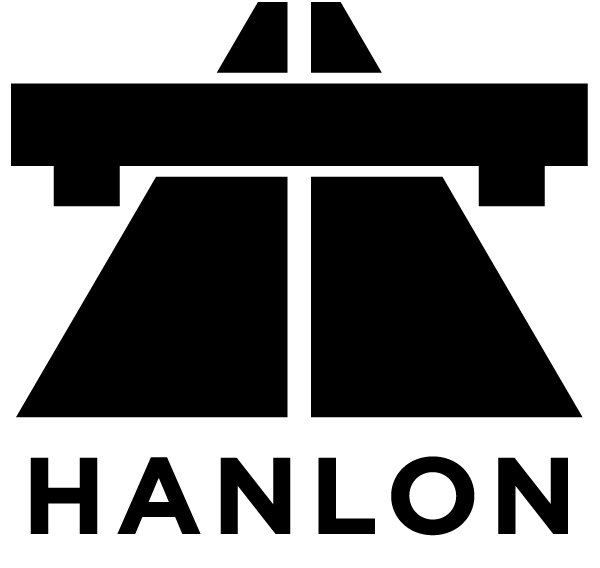
\includegraphics[height=2in]{img/hanlon-logo.png}
	%\caption{The team logo}
	\label{fig:kitten}
\end{figure}

\subsection{Team Members}
Hanlon is comprised of the following students:\\
1. \textbf{\hspace*{8pt}David DiMaria} - Project Manager\\
2. \textbf{\hspace*{8pt}Braydon Johnson} - Software Developer, User Interface Designer\\
3. \textbf{\hspace*{8pt}Joshua Lemieux} - Project Manager, User Interface Designer\\
4. \textbf{\hspace*{8pt}Neivin Mathew} - Software Developer, User Interface Designer\\
5. \textbf{\hspace*{8pt}Like Zheng} - Software Developer

\subsection{Team Roles}
\subsubsection*{Project Manager}
The Project Manager predicts potential problems that may arise during development, and plans tasks to ensure that the project is completed successfully and on time. This role involves the scheduling and unblocking of tasks. It may also involve some programming.

\subsubsection*{Software Developer}
The Developer is involved in all aspects of the software development process including research, design, coding, documentation and testing.

\subsubsection*{User Interface Designer}
The User Interface (UI) Designer role is to plan out and develop any user facing component of the system which includes the specific layout of screens, and improving the interaction between the customer and the product.

\subsection{Prototyping Session Roles}
The members of Hanlon were responsible for different aspects of the prototyping session:\\
1. \textbf{\hspace*{8pt}David DiMaria} - Mobile Application Facilitator\\
2. \textbf{\hspace*{8pt}Braydon Johnson} - Observer/Note Taker\\
3. \textbf{\hspace*{8pt}Joshua Lemieux} - Mobile Application Observer\\
4. \textbf{\hspace*{8pt}Neivin Mathew} - Web Portal Facilitator\\
5. \textbf{\hspace*{8pt}Like Zheng} - Web Portal Observer

\subsection{Team Organization}
Hanlon will follow a static team structure. Each member will maintain their respective roles for the entire duration of the project. \par

Hanlon will use a democratic majority voting system for any decisions that need to be taken within the team. Each present member will be involved in voting, and possesses one vote per motion. A motion is passed when a simple majority is achieved. \par

In the event of a team member being unavailable, and a majority cannot be established, a motion can only be passed through unanimous consent.

\clearpage
\section{Client Details and Use Cases}
\subsection{List of Use Cases}
Participants of the were split between the mobile application and the web portal:

\textbf{Mobile Application Use Cases:}\\
1.\hspace*{8pt} Create a Farmer user account\\
2.\hspace*{8pt} Login to a Farmer user account\\
3.\hspace*{8pt} Add a crop to your list of Crops\\
4.\hspace*{8pt} Harvest one of your Crops\\
5.\hspace*{8pt} Delete one of your Crops\\
6.\hspace*{8pt} Change your name in your User Profile\\
7.\hspace*{8pt} Change your Account Password\\

\textbf{Web Portal Use Cases:}\\
1.\hspace*{8pt} Login using the email "admin@aret.com" and the password "pass"\\
2.\hspace*{8pt} Create a researcher account for yourself\\
3.\hspace*{8pt} Upload research document\\
4.\hspace*{8pt} Vet a document that has already been uploaded\\
5.\hspace*{8pt} Unvet a document that has already been vetted\\
6.\hspace*{8pt} Download research\\
7.\hspace*{8pt} Find a farmer by the name of "Leia Leake"\\
8.\hspace*{8pt} Find all farmers older than 30 that live in Dowa\\
9.\hspace*{8pt} Remove the location criteria\\
10.\hspace*{3pt} Get the ARET employee Daenerys Targaryen's email address\\
11.\hspace*{3pt} Logout from system administrator

\subsection{Participants}
The prototyping session included the following three participants:\\
1.\hspace*{8pt} \textbf{Corey Alexander}\\
Corey is a Teaching Assistant (TA) in his late twenties. He asked us about our database design and sequence diagrams. Specifically, he wanted to see our tables, and inquired about why our primary keys were automatically incrementing integers. He also wondered how we would deal with holes in our database if we delete users. Regarding sequence diagrams, he asked us to draw a sequence diagram for logging in to the application. For the most part he agreed with the diagram, but wanted to us to break down the objects further.\\[0.5\baselineskip]
2.\hspace*{8pt} \textbf{Oliver Cook}\\
Oliver is a Teaching Assistant (TA) in his mid twenties, who is proficient with computers and is not representative of the client. He completed all of the use cases quite rapidly, and generally felt that the web portal prototype behaved exactly as he expected it to. He asked us about the API documentation and our technology stack.\\[0.5\baselineskip]
3.\hspace*{8pt} \textbf{Devin}\\
Devin is a Teaching Assistant (TA) in his mid twenties. He seemed to have a solid understanding of computer science related topics. He did not work through any of the use cases, but talked to the team about the deisgn and structure of the API. He asked us about our technology stack, inquired about security concerns with the API, and how we dealt with accommodating for the requirements of the mobile and web team simultaneously. \\[0.5\baselineskip]

\clearpage
\section{Things That Worked}
Overall, the response to our API (Application Programming Interface) was overwhelmingly positive. Participants thought that our API provided a proper back-end for the mobile and web teams to implement. The design of the API made sense to the participants after our team explained the design. It was difficult to accurately analyze what elements of our framework worked well, since some of the functionality that our API provided was not implemented in either the mobile application or the web portal.\par
The API provided multiple endpoints for each database table and served JSON responses over HTTPS (Hypertext Transfer Protocol Secure) for the mobile application and the web portal. The API was capable of querying the tables based on some criteria, and allowed for login, creation and updating of user accounts.\par
Our documentation was easily understood by the participants. They were able to quickly read over an API request and understand its functionality. The participants were also shown our database schema and quickly understood the system's design.\par
Going through the use cases with the mobile and web team, it was clear that our API was providing the required responses for the login/create account process for all user types, loading crop information, and creating and updating Farmer records.\par

\clearpage
\section{Things to Improve}
Although most participants found the system to be adequately functional, there were some aspects of the design that were found wanting.\par
One of our participants suggested a different approach in our database design for users. Our users were split into two tables -- Farmers and ARET Employees, which decreased the maintainability of our platform. A better way to implement the same functionality would be to have a primary User table, and then have the Farmer and ARET employees table point foreign keys to the Users table. This would make our design more extensible and allow us to easily integrate additional user types.\par
Another participant noticed we did not have code in place for the file uploading portion of our application. The web portal needs the ability to upload and download research documents and the mobile application needs to to be able to download research documents as well. This is a core piece functionality in our application, and would need to be improved upon to make our backend more complete.\par
A common request from most participants was the idea of a farmer history. Currently when you query for a list of farmers, it does not include their harvest history data. To improve this functionality, we would include the harvest history in the response.\par

\clearpage
\section{Looking to the Future}
Throughout the prototyping session, the participants made a number of suggestions about improvements that they would like to see to some features of the application. Some also wished that there were additional features for certain parts of the application.\par	
In a future version of our API we would like to add a system to allow the ARET employees to send messages/notifications to farmers. We would create a database table to upload messages that are specific to a set of farmers (region, crop they are growing, etc.), and also implement a system to send push notifications to the mobile application.\par
One of the participants noticed that we had the option to upload and download research documents, which had not been implemented for the prototyping session. Since we did not get to implement hosting and retrieving files in our API, we would need to allow certain users to be able to upload files to a web server and have a database table containing information on the file (size, link, author).\par
Another participant had some concerns about the security of our system. Currently the only security measures implemented in our system is that of hashing account passwords on the server. However, this is only done once the API has received the plain text passwords. In the future we would decide on a hashing algorithm across all the teams, and the hashing and authentication would be done on both ends. Additionally, there is no security around the API itself, so anyone with the URL can access it. In the future, we would implement a token authentication to prevent unauthorized use of the API.\par

\clearpage
\section{Individual Contributions}
\subsection{David DiMaria}
\textbf{Yes! And... Using Improv}\par
Considering I was the facilitator, and I chose to go without a script, I had to use some of the improv skills that we learned in class from The Making Box. First of all I had to make eye contact when explaining the purpose of our app and what paper prototyping is. This was a helpful skill because I needed to make sure they understood how to paper prototype, and maintaining eye contact makes it easier for them to listen to what I was saying.\par
One of the skills that I actually couldn’t use was the Yes, And… skill. The reason for this is when a participant asked for clarification on a use case, I wasn’t allowed to lead them in the right direction. As much as I wanted to lead them in the right direction with a new idea, it would have made it more difficult to determine if the system was intuitive to them. Also I explicitly wasn’t allowed to give suggestions in the paper prototype session, so I had to abandon the Yes, And… tactic for the morning. 


\clearpage
\subsection{Braydon Johnson}
\textbf{The Yes! And... Lab Demo}\par
During the lab demo I did not use any of the skills from the Yes! And… philosophy, this was because I was a note taker and did not interact with the participants at all. Honestly, I don’t believe the skills would have been that useful, previously when I talked about it they were helpful because they gave us the tools to build on other people’s ideas rather than shut them down in place of our own ideas.\par 
In the prototyping session except for the introduction it was mostly watching and listening to the client, which certainly limited the options of techniques to use especially for those of us who had no real reason to interact with the participant. While there are some tools that promote our listening skills I previously stated that I wasn’t very fond of First Letter Last Letter as it made it too hard to focus on what they were saying as a whole because I was too busy listening for the end of their sentence.


\clearpage
\subsection{Josh Lemieux}
\textbf{Yes!And...Lab Demo}\par
For our paper prototyping session, I personally did not use any of the techniques as I was the Human Computer (Beep Boop). I was not allowed to communicate with the client. I was only there to provide smooth transitions between screens following the client's’ input. There were times where my group members used a little bit of knowledge gained during the prototyping session though.\par
	The last client had some rather odd suggestions that were not typical in mobile applications. Rather than immediately shutting the idea down we thought about how that would be implemented and work in our app. It turns out that they just didn’t work out with our app, but that’s okay! By taking that time to review a suggestion that initially seems to not fit with our application, we may come to see that an odd suggestion could add benefit to our application.\par
      	A lot that we learned in the improv session is not exactly applicable to the paper prototyping session. This is because you are supposed to keep your interactions with the client to be as limited as possible. This is to get their “natural” reaction to using the application. I can see us using these techniques for our wire framing session when we are communicating more directly with the client.


\clearpage
\subsection{Neivin Mathew}
\textbf{Improv and Open-Mindedness}\par
It was rather difficult to completely apply the techniques I learned during the Improv session during the wireframing session, mostly because I was simply observing the participants of the prototyping session and taking notes detailing their interaction with the application model.\par
However, even though I did not directly interact with anyone during the session, the principles behind the "Yes!And..." philosophy did help me analyze the prototype more critically.\par 
It is easy to get invested in something when you have worked on it for a long time. You begin to look at your brainchild through rose coloured glasses and often remain oblivious to glaring errors in design. It's very hard to even accept criticism for your work, especially after you have spent hundreds of hours perfecting it. \par
However, the methods I learned in the Improv session definitely helped me keep an open mind about our design and forced me to be more flexible about possible changes. Accepting every change suggested by the user really opened my eyes to some design flaws that I would not have seen otherwise. For example, I was under the impression that our colour scheme was appropriately chosen and was perfectly readable. I was sorely mistaken, since one of our participants pointed out that our colour scheme did not pass the recommended 4.5:1 contrast ratio test for readability. Remembering the methodology of "Yes!And..." really helped me realize the importance of considering different perspectives in design, especially that of a potential user. 

		
	
\clearpage
\subsection{Like Zheng}
\textbf{Yes!And... Philosophy}\par
During the prototyping session, my role was that of observer and note taker. I was responsible for observing the user's behaviour, taking notes about how the system performs, and how the user responds as well.\par
Thus, it was not my job to talk to the participant. However, our facilitator was responsible for that. I noticed that the way our facilitator communicated with participant was much more listening than talking. This is important to minimize any influence our words would have on the participant, and allow them to give us their unbiased opinion. They can now give us a true reflection of what they are thinking.\par 
The “Yes! And… philosophy was not useful during prototyping session. It is a tool for changing ideas, and in prototyping session, we were listening to the user's ideas for most of the time. Thus, I did not find the technique helpful for the prototyping session. 

\end{document}